\documentclass{ctuthesis}
\usepackage{listings}
\usepackage{color}
\usepackage{multicol}
\usepackage{tikz}
\usetikzlibrary{shapes, angles, calc, quotes,arrows,automata, positioning}


\definecolor{dkgreen}{rgb}{0,0.6,0}
\definecolor{gray}{rgb}{0.5,0.5,0.5}
\definecolor{mauve}{rgb}{0.58,0,0.82}
\definecolor{variablesColor}{rgb}{0.66,0.46,0}

\lstdefinelanguage{JASL}{
	keywordstyle=\color{blue},
    sensitive=true, % keywords are case-sensitive
    morecomment=[l]{\%}, % l is for line comment
    morestring=[b]", % defines that strings are enclosed in double quotes
    moredelim=[is][\color{variablesColor}]{|}{|},
    basicstyle=\ttfamily,
    emph={eps},
    emphstyle=\color{mauve},
    numbers=left,
    morekeywords={DFA, NFA, ENFA, reduce, toCSV, fromCSV, toDot, toSimpleDot, accepts, toRegex, fromRegex, getExample, equals, help, helpLong, getTikzIncludes, union, intersection, kleene, concatenation, complement, execute, renameState, renameLetter},
} 

\lstdefinelanguage{JASL_snippet}{
	keywordstyle=\color{blue},
	sensitive=true,
	morecomment=[l]{\%}, % l is for line comment
    morestring=[b]", % defines that strings are enclosed in double quotes
    moredelim=[is][\color{variablesColor}]{|}{|},
    basicstyle=\ttfamily,
    emph={eps},
    emphstyle=\color{mauve},
    numbers=none,
    morekeywords={DFA, NFA, ENFA, reduce, toCSV, fromCSV, toDot, toSimpleDot, accepts, toRegex, fromRegex, getExample, equals, help, helpLong, getTikzIncludes, union, intersection, kleene, concatenation, complement, execute, renameState, renameLetter},
}

\lstset{frame=tb,
  language=JASL,
  aboveskip=3mm,
  belowskip=3mm,
  showstringspaces=false,
  columns=flexible,
  basicstyle={\small\ttfamily},
  numberstyle=\small,
  keywordstyle=\color{blue},
  commentstyle=\color{dkgreen},
  stringstyle=\color{mauve},
  breaklines=true,
  breakatwhitespace=true,
  tabsize=3
}

\ctusetup{
xdoctype = B,
xfaculty = F3,
mainlanguage = english,
titlelanguage = czech,
title-english = {Finite Automata Drawing Platform},
title-czech = {Platforma pro kreslení diagramů konečných automatů},
department-english = {Department of Cybernetics},
department-czech = {Katedra kybernetiky},
author = {Tomáš Hořovský},
supervisor = {RNDr. Marko Genyk-Berezovskyj},
supervisor-address = {TODO: FILL},
month = 1,
year = 2019,
specification-file = zadani.pdf,
}

\ctuprocess

\begin{abstract-english}
The goal of this project was to develop new coding language for description of automata and operations with them, implement interactive shell interface for executing the commands and finalize the \textbf{jautomata} library for operations on automata. The language operates the \textbf{jautomata} library and implements export of automata to various output formats including \LaTeX code to display the automaton. 
\end{abstract-english}


\begin{thanks}
I thank to my family and my supervisor for support in dire times. \ldots
%TODO FILL
\end{thanks}

\begin{declaration}
Prohlašuji, že jsem předloženou práci vypracoval samostatně a že jsem uvedl
veškeré použité informační zdroje v souladu s Metodickým pokynem o
dodržování etických principů při přípravě vysokoškolských závěrečných prací. \\
%TODO EDIT/FILL
\end{declaration}

\setlength{\parskip}{1em}

\begin{document}

\maketitle

\chapter{Introduction and motivation}
When I wrote my own material for Automata, Grammars and Language theory, I stumbled upon the problem of visualising automata in the document. I wanted fast and reliable way to draw automaton diagrams in place in code, not having to include image files to the compilation folder. I searched for a suitable way to do so and I found \textbf{tikz}. Tikz is a powerful image drawing library that has many features. I tried drawing automaton directly with tikz, but the code was unnecessarily long and tedious to write. After a couple of diagrams I started looking for another option. Then I found a library for tikz called \textbf{automata}. It was just what I was looking for. It could draw nodes and edges nicely, while keeping the code simple and clear. 

Next problem on the line was to draw these diagrams, so that they are as simple as possible. Mostly eliminating crossing edges did the trick. However the more complex the diagram got, the harder it was to eliminate those by hand. I used \textit{Graphviz} to do the layout work for me. Then it was all about the process of converting Graphviz output to the tikz code.

Automata have a few common operations associated with them. These include reduction, deciding whether $w \in L$, constructing automaton that accepts language $L = L_1 \cup L_2$ or even automaton that accepts $L^*$. I decided to create a library that would implement all of these operations and more. There are libraries that can do these operations (TODO: \href{https://gitlab.fit.cvut.cz/algorithms-library-toolkit/automata-library/}{Algorithms Library Toolkit}), but they are complicated to use and they can not output directly to \LaTeX code. 

Goal of this project is to write a program that would implement intuitive command line interface for operating my jautomata library that contains most of the commonly-used algorithms for working with automata. It would also allow the user to convert automata to various output formats including \LaTeX code.

The implemented solution uses various other programs and libraries to make the codebase smaller. It uses tools such as \textbf{Graphviz} %TODO LINK 
or \textbf{graphviz-java} %TODO LINK 
library. Sometimes it was not so easy to work with these libraries, because their actual purpose for this project was different from their intended use. More on that in chapter %TODO Link

TODO: CONTINUE

\chapter{User manual}
\section{Installation}
There are two ways of installing this program. You can either download pre-compiled .jar file or compile your own. If you just want to use the program, skip the next section right to the running section~\ref{sec:execution}

\subsection{Compiling JAR yourself}
If you want to compile it yourself, you have to get source code of the project from repository: https://github.com/horovtom/jautomata %TODO Interactive link
After, you can install it using Maven and JDK. %TODO Link

Open console in the root directory of the downloaded project and run these commands:
\begin{verbatim}
	mvn clean
	mvn install
\end{verbatim}

After building the project, you can find the compiled .jar file in the target folder. Use the compiled .jar with dependencies.

\section{Execution}
\label{sec:execution}
The program can be executed from the console with this command:

\begin{verbatim}
	java -jar <path-to-jar> <args>
\end{verbatim}

If no args are specified, the program will enter interactive shell mode where you can type your commands and get immediate response for every command. The shell will store user variables to memory and user can use them freely. However after terminating the shell environment (by using command: \textbf{quit}) all saved variables are lost. We can achieve the same effect without closing the environment by using command \textbf{clear}. 

If switch -f is specified, the program will look for its argument, which should be the path to an existing file. JASL will then execute commands from this file line by line. Note, that all variables are lost after terminating the program. 

User can execute file from shell, where the interpreter will use variables in current session. This can be done by using execute function~\ref{subsec:execute}. 

\section{Syntax of the language}
The \textbf{JASL} language allows the user to define variables and call functions upon those variables. The commands are parsed line by line. On every line there is one assignment or a command. 

Function calls consist of the name of the function followed by a comma-separated arguments enclosed in a pair of parentheses.

We can comment JASL code with line comments. Every line comment starts with \textbf{\%} sign. Everything that follows the percent sign will not be parsed and the whole line will be skipped. 

Help for the JASL syntax can be displayed with command \textbf{help} while \textbf{helpLong} prints longer, more detailed version with descriptions of functions. 
%TODO CHECK AND FILL MBY

\subsection{Functions}
In this section we will describe in detail the functions that are implemented to JASL syntax.

\subsubsection{execute}
\label{subsec:execute}
\begin{lstlisting}[language = JASL_snippet]
	execute(file.jasl)
\end{lstlisting}

This function will execute script on specified path. It will use currently defined variables for the execution and update them.

\subsubsection{fromCSV}
\begin{lstlisting}[language = JASL_snippet]
	|$automaton| = fromCSV(file.csv)
\end{lstlisting}

This function will return new Automaton object, loaded from comma-separated csv file specified in the single argument of this function. The CSV output/input format is specified in greater detail in chapter: TODO.

\subsubsection{getExample}
\begin{lstlisting}[language = JASL_snippet]
	|$automaton| = getExample()
\end{lstlisting}

This function will get example automaton. This automaton is described by table:
\begin{table}[H]
\begin{ctucolortab}
\begin{tabular}{cc|c|c}
	 & & $a$ & $b$ \\\Midrule
	$\rightarrow$ & $0$ & $1$ & $2,3$ \\
	$\rightarrow$ & $1$ & & $1,4$ \\
	$\leftrightarrow$ & $2$ & & $0$ \\
	$\leftarrow$ & $3$ & $3$ & $3$ \\
	 & $4$ & $4$ & $2$ 
\end{tabular}
\end{ctucolortab}
\caption{Transition table of example automaton}
\label{fig:example_automaton_table}
\end{table}

And it's state diagram:
\begin{figure}[H]
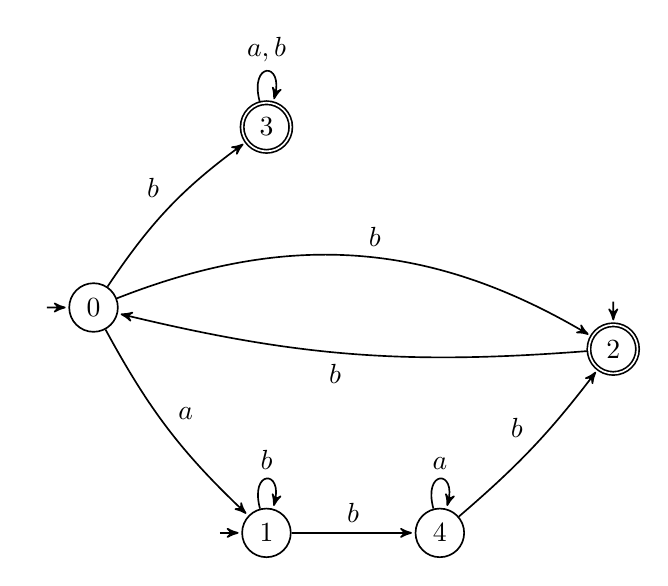
\begin{tikzpicture}[->,>=stealth',shorten >=1pt,auto,node distance=2.8cm,semithick,initial text=$ 	$, scale=0.6]
	\tikzset{every state/.style={minimum size=0pt}}
	\node[state, initial, initial where=left] (0) at (4.51,5.46) {$0$};
	\node[state, initial, initial where=left] (1) at (8.17,0.69) {$1$};
	\node[state, initial, initial where=above, accepting] (2) at (15.51,4.58) {$2$};
	\node[state, accepting] (3) at (8.17,9.28) {$3$};
	\node[state] (4) at (11.84,0.69) {$4$};
	\path
		(0)

			edge [bend right = 9] node {$a$} (1)
			edge [bend left = 26] node {$b$} (2)
			edge [bend left = 10] node {$b$} (3)
		(1)

			edge [loop above] node {$b$} (1)
			edge  node {$b$} (4)
		(2)

			edge [bend left = 9] node {$b$} (0)
		(3)

			edge [loop above] node {$a,b$} (3)
		(4)

			edge [bend right = 6] node {$b$} (2)
			edge [loop above] node {$a$} (4);
\end{tikzpicture}
\caption{State diagram of the example automaton}
\label{fig:example_automaton_diagram}
\end{figure}

\subsubsection{fromRegex}
\begin{lstlisting}[language = JASL_snippet]
	|$automaton| = fromRegex(a*b(a+b)*)
\end{lstlisting}

This function will return new Automaton object specified by regular expression passed in as an argument. The regular expression will be in format specified in chapter: TODO.

There are limitations of this function. It will work only with single characters long letters. Characters can not be escaped, so symbols '\textbf{(}', '\textbf{)}' and '\textbf{*}' can not be used as letters.

\subsubsection{getTikzIncludes}
\label{subsec:getTikzIncludes}
\begin{lstlisting}[language = JASL_snippet]
	getTikzIncludes()
\end{lstlisting}

This will output a couple lines of \TeX code includes, needed for the Tikz diagrams to work.

\subsection{Defining a variable}
Variables are defined as follows:
\begin{lstlisting}[language = JASL_snippet]
	|$variableName| = value
\end{lstlisting}

Variable name can be any string that does not contain '$\$$', '$\ $' or '$.$'. Variables can hold objects of these types:
\begin{itemize}
	\item string - \verb'$thisIsString = hello world'
	\item list - \verb'$thisIsList = {a, b, c}'
	\item automaton - \verb'$thisIsAutomaton = ENFA($args)'
\end{itemize}

Now we will look at the details of defining lists and automata:

\subsubsection{Defining lists}
Lists are enclosed in pairs of curly brackets. Elements are separated by commas. Elements can be any objects or variables. Lists can be empty and they can be nested. They are used for defining automata. Some examples of lists:

\begin{minipage}{\linewidth}
\begin{lstlisting}[language = JASL_snippet]
	{a, b, c}
	{}
	{a, {b, {}}, c}
\end{lstlisting}
\end{minipage}
TODO: Check and complete

\subsubsection{Defining automata}
JASL implements these types of automata:

\begin{itemize}
	\item DFA (deterministic finite automaton)
	\item NFA (non-deterministic finite automaton)
	\item ENFA (epsilon non-deterministic finite automaton)
\end{itemize}

To define an automaton we need to use the constructor function. This function accepts one parameter. This parameter is the transition table of the automaton, enclosed in nested list. Elements of this list are:

\begin{enumerate}
	\item The alphabeth $\Sigma$ as an ordered list of letters.
	\item $|Q|$ lists. For every state $q \in Q$ we define a list as such:
		\begin{enumerate}
			\item Whether $q$ is an initial state $q \in I$ (denoted by '<') or whether $q$ is a final state $q \in F$ (denoted by '>') or both (denoted by '<>'). If $q \not \in (I \cup F)$, then we can skip this field and not append it to the list whatsoever.
			\item The name of the state $q$.
			\item For every letter $l \in \Sigma$ we append a list of target states $q \in Q$.
		\end{enumerate}
\end{enumerate}

Basically lists in the definition are the rows of transition table read from left to right, separated by commas.

Example conversion:
\begin{table}[H]
\begin{ctucolortab}
\begin{tabular}{cc|cc}
	&	& $a$	& $b$ \\\Midrule
$\leftrightarrow$	& $0$	& $\emptyset$	& $2$ \\
$\rightarrow$	& $1$ & $0$ & $1,2$ \\
$\leftarrow$	& $2$ & $1,2,3$ & $1$ \\
				& $3$ & $3$	& $\emptyset$ 
\end{tabular}
\quad
$\rightarrow$
\begin{tabular}{|c|c|c|c|}
\hline
	&&$a$&$b$ \\
	$<>$ & $0$ & $\{\}$ & $2$ \\
	$>$ & $1$ & $0$ & $\{1,2\}$ \\
	$<$ & $2$ & $\{1,2,3\}$ & $1$ \\
		& $3$ & $3$ & $\{\}$\\
		\hline
\end{tabular}
\quad 
$\rightarrow$
\begin{tabular}{|l|}
\hline 
$\{a, b\}$ \\
$\{<>,0,\{\}, 2\}$ \\
$\{>,1,0,\{1,2\}\}$ \\
$\{<,2,\{1,2,3\},1\}$ \\
$\{3, 3, \{\}\}$ \\\hline
\end{tabular}
\end{ctucolortab}
\caption{Example of conversion of trasition table to list}
\label{fig:example_conversion}
\end{table}

So the argument to construct this automaton is:
\begin{lstlisting}[language = JASL_snippet]
	{{a,b},{<>,0,{},2},{>,1,0,{1,2}},{<,2,{1,2,3},1},{3,3,{}}}
\end{lstlisting}

The automaton specified by the transition table is a NFA automaton. So we create this automaton with respective constructor function. For clarity we can split the definition of the nested list into multiple list variables. 

\begin{minipage}{\linewidth}
\begin{lstlisting}[language = JASL]
	|$alphabeth| = {a, b}
	|$row0|  = {<>,0,{},2}
	|$row1|  = {>,1,0,{1,2}}
	|$row2|  = {<,2,{1,2,3},1}
	|$row3|  = {3,3,{}}
	
	% Now we can define the nested list:
	|$nestedList| = {|$alphabeth|, |$row0|, |$row1|, |$row2|, |$row3|}
    
	% And now we can define an automaton:
	|$automaton| = NFA(|$nestedList|)
\end{lstlisting}
\end{minipage}

\paragraph{Note about ENFA automata}
ENFA automata can have $\varepsilon$-transitions. We mark these as another letter of the alphabeth. The letter \textbf{eps}. So the alphabeth of ENFA automaton could be:
\begin{lstlisting}[language = JASL]
	|$alphabeth| = {eps, a, b}
\end{lstlisting} 

\subsection{Member functions}
We can call member functions of objects saved in variables. Member functions are defined for automata objects. We call these member functions like this:
\begin{minipage}{\linewidth}
\begin{lstlisting}[language = JASL_snippet]
	|$result| = |$automaton|.functionName(|$arg1|, |$arg2|)	
\end{lstlisting}
\end{minipage} 

Note that we can chain member function calls on one line:

\begin{minipage}{\linewidth}
\begin{lstlisting}[language = JASL]
	|$reduced| = |$automaton|.reduced()
	|$reduced|.toPNG(image.png)
	
	% Can be written as:
	|$automaton|.reduced().toPNG(image.png)
\end{lstlisting}
\end{minipage}

Now we will list all member functions for automata objects:

\subsubsection{accepts}
\begin{lstlisting}[language = JASL_snippet]
	|$M|.accepts(aabbaab)
\end{lstlisting}

This function returns \textit{true} if automaton $M$ accepts word passed in argument ($w \in L(M)$). It outputs \textit{false} otherwise. The argument of this function can be a string or a list of letters. Note, that if you have an automaton that has letters with more than one character, variant with argument of type string will not work. In that case you need to use list as an argument.

\subsubsection{equals}
\begin{lstlisting}[language = JASL_snippet]
	|$M1|.equals(|$M2|)
\end{lstlisting}

This function returns \textit{true} if $L(M1) = L(M2)$. It outputs \textit{false} otherwise. In other words this function checks, whether two automata accept the same language. 

\subsubsection{reduce}
\begin{lstlisting}[language = JASL_snippet]
	|$M2| = |$M|.reduce()
\end{lstlisting}

This function returns reduced automaton $M2$. Note that this function creates a new automaton object, so the original automaton remains unchanged.

\subsubsection{toCSV}
\begin{lstlisting}[language = JASL_snippet]
	|$M|.toCSV(m.csv)
\end{lstlisting}

This function creates/overwrites csv file on path specified by the argument. The csv will contain description of the automaton in format, that is specified in chapter: TODO

\subsubsection{toPNG}
\begin{lstlisting}[language = JASL_snippet]
	|$M|.toPNG(m.png, circo)
\end{lstlisting}

This function creates/overwrites png file on path specified by the argument. The png will contain image of the state diagram of the automaton $M$. 

The second argument to toPNG is optional. It is the layout (engine) that Graphviz will use to organize the graph. When no layout is specified, \textbf{dot} will be used as a default. Possible layouts are: \textbf{circo}, \textbf{neato}, \textbf{dot}.

\subsubsection{toTexTable}
\begin{lstlisting}[language = JASL_snippet]
	|$M|.toTexTable()
\end{lstlisting}

This function will output string containing \TeX code to display the transition table of automaton $M$. 

\subsubsection{toRegex}
\begin{lstlisting}[language = JASL_snippet]
	|$M|.toRegex()
\end{lstlisting}

This function will output regular expression describing language $L = L(M)$. Because no regular expression simplifier is implemented, the output of this function can be quite complicated. Nevertheless, it describes the language $L$.

\subsubsection{toDot}
\label{subsec:toDot}
\begin{lstlisting}[language = JASL_snippet]
	|$M|.toDot(neato)
\end{lstlisting}

This function will output dot code, that contains description of the automaton state-diagram image. It accepts one, optional argument. The argument is the layout (engine) that Graphviz will use to organize the graph. When no layout is specified, \textbf{dot} will be used as a default. Possible layouts are: \textbf{circo}, \textbf{neato}, \textbf{dot}. 

TODO: THIS IS JUST A COPY OF THE ABOVE TEXT! DEAL WITH IT?

\subsubsection{toSimpleDot}
\begin{lstlisting}[language = JASL_snippet]
	|$M|.toSimpleDot()
\end{lstlisting}

This function will output dot code, that contains description of the automaton state-diagram image. As opposed to toDot~\ref{subsec:toDot}, the dot code will not contain positions of elements, because it has not been run through Graphviz yet. 

\subsubsection{toTikz}
\begin{lstlisting}[language = JASL_snippet]
	|$M|.toTikz(dot)
\end{lstlisting}

This function will output Tikz code to display the state diagram of automaton $M$. It accepts one parameter, that is the layout (engine) graphviz will use to organize the graph. When no layout is specified, \textbf{dot} will be used as a default. Possible layouts are: \textbf{circo}, \textbf{neato}, \textbf{dot}. It is recommended to not specify this argument (hence use dot as an engine), because it will generally output the nicest results. Note that you need to add appropriate includes to your \TeX code. You can get these using getTikzIncludes~\ref{subsec:getTikzIncludes}.

\subsubsection{union}
\begin{lstlisting}[language = JASL_snippet]
	|$M3| = |$M1|.union(|$M2|)
\end{lstlisting}

This member function accepts one other automaton. It will output new automaton $M_3$ that accepts union of languages accepted by automata $M_1, M_2$. 
\begin{equation*}
L(M_3) = L(M_1) \cup L(M_2)
\end{equation*}

\subsubsection{intersection}
\begin{lstlisting}[language = JASL_snippet]
	|$M3| = |$M1|.intersection(|$M2|)
\end{lstlisting}

This member function accepts one other automaton. It will output new automaton $M_3$ that accepts intersection of languages accepted by automata $M_1, M_2$.
\begin{equation*}
	L(M_3) = L(M_1) \cap L(M_2)
\end{equation*}

\subsubsection{kleene}
\begin{lstlisting}[language = JASL_snippet]
	|$M2| = |$M1|.kleene()
\end{lstlisting}

This member function will output new automaton $M_2$ such that:
\begin{equation*}
	L(M_2) = L(M_1)^*
\end{equation*}

\subsubsection{complement}
\begin{lstlisting}[language = JASL_snippet]
	|$M2| = |$M1|.complement()
\end{lstlisting}

This function will return automaton that accepts language, that is the complement to the language of the original automaton.
\begin{equation*}
	L(M_2) = \overline{L(M_1)}
\end{equation*}

\subsubsection{concatenation}
\begin{lstlisting}[language = JASL_snippet]
	|$M3| = |$M1|.concatenation(|$M2|)
\end{lstlisting}

This function accepts one other automaton as a parameter. It will output new automaton $M_3$ that accepts the concatenation of languages accepted by automata $M_1, M_2$.
\begin{equation*}
	L(M_3) = L(M_1)L(M_2)
\end{equation*}


\subsubsection{renameState}
\begin{lstlisting}[language = JASL_snippet]
	|$M1|.renameState(0, 2a)
\end{lstlisting}

This function accepts two arguments. The old state name as first and the new one as second argument. It will fail if the original state has not been found in the automaton or if the new name is already taken by some other state of the automaton.


\subsubsection{renameLetter}
 \begin{lstlisting}[language = JASL_snippet]
	|$M1|.renameLetter(a, css)
\end{lstlisting}

This function accepts two arguments. The old letter name as first and the new one as second argument. It will fail if the original letter has not been found in the automaton or if the new name is already taken by some other letter of the automaton.

\chapter{Details of Implementation}
TODO: FILL

\chapter{Drawing images - details}
TODO: FILL

\chapter{Examples of usage, practice, problems of testing}
Here are some examples of usage of the \textbf{JASL} language: 

\section{Defining a NFA automaton}
\label{sec:example_NFA}
Suppose we have regular language: 
\begin{equation*}
L_1 = \{w \mid w \text{ contains } aba \text{ as substring }\}, L_1 \subseteq \{a, b\}^*
\end{equation*} 
We design regular automaton $M$ such that $L(M) = L_1$. Example of such automaton could be this non-deterministic automaton:
\begin{table}[H]
\begin{ctucolortab}
\begin{tabular}{cc|cc}
\multicolumn{2}{c}{\bfseries $M_1$} & \bfseries $a$ & \bfseries $b$ \\\Midrule
$\rightarrow$ 	& $0$ & $0,1$ 	& $0$  \\
				& $1$ &  	& $2$  \\
				& $2$ & $3$		&  \\
$\leftarrow$	& $3$ & $3$		& $3$ 
\end{tabular}
\end{ctucolortab}
\caption{Transition table of automaton $M_1$.}
\label{fig:examples_NFA_table}
\end{table} 

In order to define automaton $M_1$ in JASL language we have to define a few lists: 

\begin{minipage}{\linewidth}
\begin{lstlisting}[language = JASL]
	|$alphabeth| = {a, b}
	|$row0|  = {>, 0, {0,1}, 0}
	|$row1|  = {1, {}, 2}
	|$row2|  = {2, 3, {}}
	|$row3|  = {<, 3, 3, 3}
    
	% Now we can define an automaton:
	|$M_1|  = NFA({|$alphabeth|, |$row0|, |$row1|, |$row2|, |$row3|})

	% We can get, whether automaton accepts word bbbbaab:
	|$accepted| = |$M_1|.accepts(bbbbaab)   
	% Accepted has value: false 
	
	% We can get regular expression describing the language L1:
	|$reg| = |$M_1|.getRegex()
	% $reg has value: b*aa*b((bb*aa*b)*)a((a+b)*) 

	% But does this regex really describe language L1? 
	% This one definitely does:
	|$regex| = (a+b)*aba(a+b)*
	|$M_2| = fromRegex($regex)
	|$M_2|.equals(|$M_1|) 	
	% Outputs: true
\end{lstlisting}
\end{minipage}

Note that we use nested lists for definitions of sets of target states. We can use $\{\}$ to denote $\emptyset$. The output of .getRegex() can be quite complicated. That is because no real regular expression simplifier has been implemented yet.

\section{Defining an ENFA automaton}
\label{sec:example_ENFA}
Suppose we have a ENFA automaton $M_2$ that accepts language L such that:
\begin{equation*}
	\underline{r} = a^*+b^*, \hspace{1cm} L_{\underline{r}} = L = L(M_2) 
\end{equation*}
Such automaton can be described by this transition table:
\begin{table}[H]
\begin{ctucolortab}
\begin{tabular}{cc|ccc}
\multicolumn{2}{c}{$M_2$} & $\varepsilon$ & $a$ & $b$ \\\Midrule
$\rightarrow$ 	& $S$ & $A,B$  \\
				& $A$ & $F$ 	& $A$  \\
				& $B$ & $F$		& & $B$ \\
$\leftarrow$	& $F$ & 		&  
\end{tabular}
\end{ctucolortab}
\caption{Transition table of automaton $M_2$.}
\label{fig:examples_DFA_table}
\end{table} 

We can define this automaton in JASL as such:

\begin{minipage}{\linewidth}
\begin{lstlisting}[language = JASL]
	|$Sigma| = {eps, a, b}
	% We can even shorten the definition by the last empty transitions
	|$stateS| = {>, S, {A, B}}
	|$stateA| = {A, F, A}
	|$stateB| = {B, F, {}, B}
	|$stateF| = {<, F}
	|$M_2| = ENFA({|$Sigma|, |$stateS|, |$stateA|, |$stateB|, |$stateF|})
	
	% Now we can save png image of automaton M_2:
	|$M_2|.toPNG(image.png)	
\end{lstlisting}
\end{minipage}

The resulting image is:

\begin{figure}[H]
\includegraphics[width=0.8\linewidth]{figures/ENFA_definition.png}
\caption{Image saved in image.png}
\label{fig:ENFA_definition_example}
\end{figure}

\section{Example of Tikz image}
Suppose we have automaton $M_3$. This automaton accepts language $L = L(M_3)$. This language is also described by regular expression $\underline{r_2}$. 
\begin{equation*}
	\underline{r_2} = (a+b)^*ab^*, \hspace{1cm} L(M_3) = L_{\underline{r_2}} = L
\end{equation*}

We construct this automaton and create tex file to display it in JASL:

\begin{minipage}{\linewidth}
\begin{lstlisting}[language = JASL]
	|$a| = fromRegex((a+b)*ab*)
	% Tex document parts
	|$class| = \documentclass{article}
	|$includes| = getTikzIncludes()
	|$beginning| = \begin{document}
	|$tikzCode| = |$a|.toTikz()
	|$end| = \end{document}
	
	% Now save these parts to image.tex file
	|$class|.save(image.tex)
	|$includes|.save(image.tex)
	|$beginning|.save(image.tex)
	|$tikzCode|.save(image.tex)
	|$end|.save(image.tex)
\end{lstlisting}
\end{minipage}

After compiling image.tex file we get this image:

\begin{figure}[H]
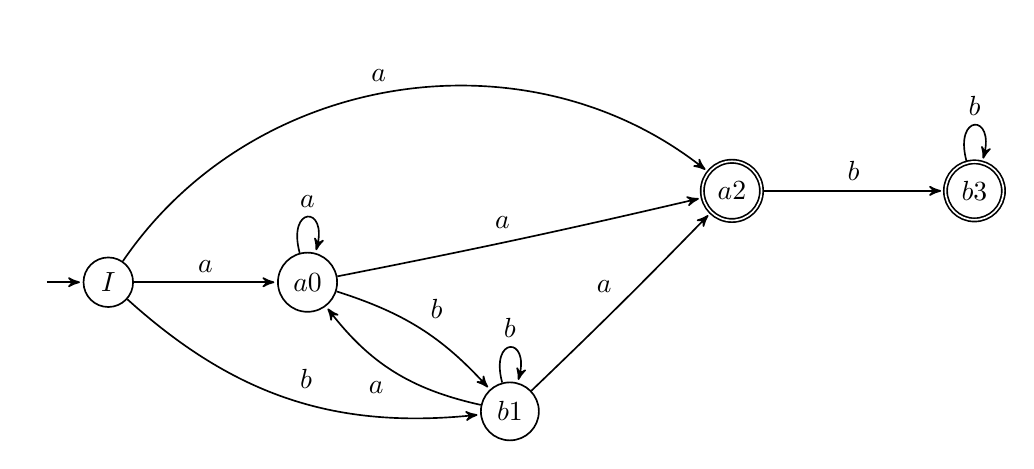
\begin{tikzpicture}[->,>=stealth',shorten >=1pt,auto,node distance=2.8cm,semithick,initial text=$ 	$]
	\tikzset{every state/.style={minimum size=0pt}}
	\node[state] (0) at (5.97,2.26) {$a0$};
	\node[state] (1) at (8.54,0.62) {$b1$};
	\node[state, accepting] (2) at (11.36,3.42) {$a2$};
	\node[state, accepting] (3) at (14.44,3.42) {$b3$};
	\node[state, initial, initial where=left] (4) at (3.44,2.26) {$I$};
	\path
		(0)

			edge [loop above] node {$a$} (0)
			edge [bend left = 15] node {$b$} (1)
			edge [bend right = 1] node {$a$} (2)
		(1)

			edge [bend left = 20] node {$a$} (0)
			edge [loop above] node {$b$} (1)
			edge [bend right = 1] node {$a$} (2)
		(2)

			edge  node {$b$} (3)
		(3)

			edge [loop above] node {$b$} (3)
		(4)

			edge  node {$a$} (0)
			edge [bend right = 24] node {$b$} (1)
			edge [bend left = 47] node {$a$} (2);
\end{tikzpicture}
\caption{Image in compiled image.pdf file.}
\label{fig:compilation_tikz_code}
\end{figure}

\section{Example of executable file}

Suppose we have a file append.jasl, that contains the code that will concatenate regular expression: $ab^*a$ to language accepted by automaton saved in variable \textbf{\$i}. It will save the result to variable \textbf{\$j}. Such file could contain for example this code:

\begin{minipage}{\linewidth}
\begin{lstlisting}[language = JASL]
	|$append| = fromRegex(ab*a)
	|$j| = |$i|.concatenation(|$append|)
\end{lstlisting}
\end{minipage}

We can check whether the function worked correctly:

\begin{minipage}{\linewidth}
\begin{lstlisting}[language = JASL]
	|$i| = fromRegex(bba)
	execute(append.jasl)
	|$shouldBe| = fromRegex((bba)(ab*a))
	|$j|.equals(|$shouldBe|)
\end{lstlisting}
\end{minipage} 

The last command will print true to console. Note that by executing code in append.jasl we have overwritten anything that might be in the variable \$append. The user has to be aware of this side effect. Stack frames might be implemented later~\ref{subsec:stack_frames}

\chapter{What to do next? Looking to the future}
TODO: FILL


\chapter{Conclusion}
Lorep ipsum \cite{doe}

\begin{thebibliography}{1}
\bibitem{doe} J. Doe. \emph{Book on foobar.} Publisher X,
2300.
\end{thebibliography}

\end{document}

%\begin{figure}
%\includegraphics[width=0.8\linewidth]{mygraphicfile.pdf}
%\caption{We depict a foo-bar here.}
%\label{fig:foobar}
%\end{figure}

%\begin{table}
%\begin{ctucolortab}
%\begin{tabular}{cc}
%\bfseries Foo & \bfseries Bar \\\Midrule
%foo1 & bar1 \\
%foo2 & bar2
%\end{tabular}
%\end{ctucolortab}
%\caption{Table of foo-bar.}
%\label{tab:foobar}
%\end{table}
